% Copyright (c) 2022 Hans Wan, Chiro Liang and ReiSakuma
% All rights reserved.
% This paper is publicised for non-commercial learning purpose only.
% THIS PAPER IS PROVIDED ON AN "AS IS" BASIS, WITHOUT WARRANTIES OF ANY KIND,
% EITHER EXPRESS OR IMPLIED, INCLUDING BUT NOT LIMITED TO NON-INFRINGEMENT,
% MERCHANTABILITY OR FIT FOR A PARTICULAR PURPOSE.

\documentclass[a4paper]{article}
\usepackage{hcr-cumcm}
\usepackage[style=gb7714-2015,backend=biber]{biblatex}
\addbibresource{bibdata.bib}
\title{基于生物躯体水平形态的时间控制方法研究}

\begin{document}
    \pagestyle{plain}
    \maketitle

    %% ABSTRACT
    \section*{摘要}

哼哼,啊啊啊啊啊啊啊啊啊啊啊啊啊啊啊

    %% CONTENT
    \section{问题重述}

\subsection{问题背景}
在全球推进新能源发展的环境下,波浪能作为一种清洁无污染的可再生能源,既可降低石油开采量、节约资源,又可减少二氧化碳排放,是应对能源短缺以及环境问题,发展清洁能源、调整能源结构的重要选择之一。

我国波浪能资源丰富,可开发利用程度高,因此开发波浪能资源对解决我国资源问题具有重大意义。
同时,近些年来,波浪能利用已经成为全球范围的研究热点,波浪能发电装置种类繁多,层出不穷,各国学者都在积极探索高效转换能量的波浪装置和装置的分析方法。
本题所描述的就是一种摇荡式波能转换装置,它由一个外部「浮子」壳体和内部「振子」块体所构成,通过装置漂浮时浮子和振子之间产生的相对运动来驱动阻尼器做功,实现能量的捕获和转换。

\subsection{问题要求}

\subsubsection{问题一}

此题只考虑浮子在波浪中做垂荡运动的情况,要求建立浮子与振子的运动模型,根据题目所给出的参考值,分别针对直线阻尼器的阻尼系数的两种不同情况,计算浮子和振子在波浪激励力的作用下各个时间点的垂荡位移和速度。

\subsubsection{问题二}

此题仍只考虑浮子在波浪中只做垂荡运动的情况,同样分别针对上题的两种情况,建立确定最优阻尼系数的数学模型,使得输出功率最大,并计算出输出功率和最优阻尼系数的具体结果。

\subsubsection{问题三}

此题在垂荡运动基础上加入纵摇运动,规定扭转弹簧的扭矩与浮子和振子的相对角速度成正比,比例系数为旋转阻尼器的旋转阻尼系数。
考虑浮子同时做垂荡和纵摇运动时的情况,规定直线阻尼器和旋转阻尼器的阻尼系数为常量,要求建立浮子与振子的运动模型,计算浮子和振子在波浪激励力的作用下各个时间点时的垂荡位移和速度。

\subsubsection{问题四}

此题亦考虑浮子同时垂荡和纵摇运动,规定直线阻尼器和旋转阻尼器的阻尼系数为常量,要求建立确定两个最优阻尼系数的数学模型,使得输出功率最大,并计算出输出功率和最优阻尼系数的具体结果。



    \section{问题分析}

下面我们对各问题进行简要的分析,为进一步的模型建立做好准备。

\subsection{问题一的分析}

问题一描述了一个在波浪中做垂荡运动的浮子模型。
对浮子进行分析,其除了受到重力、浮力外,还直接受到波浪产生的激励力以及海水带来的附加惯性力、兴波阻尼力和静水恢复力。
而在内部,浮子还受到由理想弹簧和阻尼器构成的能量输出系统(简称 PTO)产生的拉(推)力和阻尼力。
同时,对振子进行分析,其受到的力则有重力和 PTO 的推(拉)力与阻尼力。
我们可以通过对浮子和振子进行竖直方向的受力分析,以浮子和振子的位移作为变量,列出它们的微分方程组,借助计算机进行求解,从而得到任意时刻浮子和振子的位移和速度。

在进行受力分析的过程中,为了使问题简化,我们可以将一些力进行合并、等效,从而大幅度降低分析和求解的难度。
在求解微分方程方面,我们使用 Wolfram Engine for Developers 软件\footnote{即 Wolfram Mathematica 软件的免费版本。}进行数值求解。

\subsection{问题二的分析}

问题二建立在问题一的基础之上。
对阻尼器进行分析,我们容易通过先前得到的浮子、振子位移和速度,得到任意时刻阻尼器上的相对速度,进而计算出阻尼器产生的阻尼力。
再对这些「瞬时功率」进行累加积分,容易计算出阻尼器在一段时间内的瞬时功率。
我们通过编写 Python 程序实现一种类「随机梯度下降」的算法,求解出瞬时功率在题目给定范围内的最优值。

\subsection{问题三的分析}

问题三在问题一的简单垂荡模型之上,加入了本质为绕轴旋转的纵摇运动。
浮子和振子的摆动角度作为新的变量被引入。
为了统一场景便于计算,我们建立一个统一的直角坐标系,将考虑到的各浮子和振子运动纳入其中表示。
我们在 $x$ 和 $z$ 两个方向对各种力进行分解求和,列出与浮子和振子的位移和角度有关的微分方程,再采用与问题一类似的方法进行分析求解。

\subsection{问题四的分析}

问题四与问题二类似,需要计算平均功率。
由于问题三已经计算出各个时刻的浮子、振子状态,我们也需要计算一系列瞬时功率,并进行累加积分,即可得到相应工况下的平均功率。
我们使用与问题二相似的方法,寻找最优的工作条件。
    \section{模型假设}

为了简化模型,便于求解,我们作出如下的假设:

\begin{enumerate}
    \item 浮子壳体和振子的质量都是均匀分布的,中轴、底座、隔层的质量为零,且对应的直径或厚度可以忽略不计。
    \item 所有摩擦都可以忽略不计,所有弹簧均是理想的并符合胡克定律,阻尼器的能量转换效率为 $100\%$。
    \item 装置在做垂荡运动时,垂荡方向严格与铅直方向平行,波浪激励力无损耗、竖直地作用在浮子上。
    \item 装置在做纵摇运动时,浮子壳体做以其浮心为轴心的旋转运动,振子做以转轴绞链为轴心的旋转运动,波浪激励力矩无损耗地作用在浮子上。
\end{enumerate}
    \section{符号说明}

在表 \ref{symbols} 中,我们约定了文中出现的各数学符号的含义和它们的单位。

\begin{table}[htbp]
    \centering
    \begin{tabular}{ccc}
        \toprule
        符号 & 含义 & 单位 \\
        \midrule
        $M$ & 浮子的质量 & $\mathrm{kg}$ \\
        $m$ & 振子的质量 & $\mathrm{kg}$ \\
        $m_0$ & 浮子受到的附加质量 & $\mathrm{kg}$ \\
        $g$ & 重力加速度 & $\mathrm{m}/\mathrm{s}^2$ \\
        $k$ & 弹簧的刚度系数 & $\mathrm{N}/\mathrm{m}$ \\
        $k_\text{rot}$ & 扭转弹簧刚度 & $\mathrm{N}\cdot\mathrm{m}$ \\
        $c$ & 阻尼器的阻尼系数 & $\mathrm{N}\cdot\mathrm{s}/\mathrm{m}$ \\
        $c_\text{rot}$ & 旋转阻尼器的阻尼系数 & $\mathrm{N}\cdot\mathrm{m}\cdot\mathrm{s}$ \\
        $c_0$ & 垂荡兴波阻尼系数 & $\mathrm{N}\cdot\mathrm{s}/\mathrm{m}$ \\ 
        $c_\text{r0}$ & 纵摇兴波阻尼系数 & $\mathrm{N}\cdot\mathrm{m}\cdot\mathrm{s}$ \\
        $I_A$ & 浮子的转动惯量 & $\mathrm{kg}\cdot\mathrm{m}^2$ \\
        $I_B$ & 振子的转动惯量 & $\mathrm{kg}\cdot\mathrm{m}^2$ \\
        $I_0$ & 纵摇附加转动惯量 & $\mathrm{kg}\cdot\mathrm{m}^2$ \\
        $M_\text{rec}$ & 静水恢复力矩系数 & $\mathrm{N}\cdot\mathrm{m}$ \\
        $F$ & 波浪激励力 & $\mathrm{N}$ \\
        $M_\text{wave}$ & 波浪激励力矩 & $\mathrm{N}\cdot\mathrm{m}$ \\
        $\omega$ & 波浪频率 & $\mathrm{s}^{-1}$ \\
        \bottomrule 
    \end{tabular}
    \caption{本文中出现的数学符号和它们的单位}
    \label{symbols}
\end{table}

    \section{模型建立与求解}

\subsection{问题一}

\subsubsection{模型的构建和分析}

在开始之前,我们需要先构建整个装置的物理模型。
以海平面为参考系。

当装置在水中静止时,对质量为 $m$ 的振子进行受力分析,则其受到的重力和受到弹簧弹力合力为零。
记以铅直向上为正方向,重力加速度为 $g$,记此时振子位移为 0,记此时弹簧压缩量为 $x_0$,弹簧的刚度为 $k$,则有 
\begin{equation}
    kx_0-mg=0 
    \label{oscilator}
\end{equation}

考虑在 $t$ 时刻,浮子位移 $x_1$,振子位移 $x_2$,正方向同前定义。
记阻尼器的阻尼系数为 $c$,对振子受力分析,如图 \ref{force-analysis} 左所示。我们有
\begin{equation}
    m\dfrac{\dif^2x_2}{\dif t^2}=k(x_1-x_2+x_0)+c(\dfrac{\dif{x_1}}{\dif{t}}-\dfrac{\dif{x_2}}{\dif{t}})-mg
\end{equation}
其中,$\dfrac{\dif^2 x_i}{\dif t^2}$ 即为瞬时加速度,$\dfrac{\dif x_i}{\dif t}$ 即为瞬时速度。

与此同时,我们对浮子进行受力分析,如图 \ref{force-analysis} 右所示。
记海水的兴波阻尼系数为 $c_0$,附加质量为 $m_0$,浮子质量为 $M$,波浪激励力为 $F$,有 
\begin{equation}
    M\dfrac{\dif^2x_1}{\dif t^2}=F+F_\text{浮}-Mg-k(x_1-x_2+x_0)-c(\dfrac{\dif{x_1}}{\dif{t}}-\dfrac{\dif{x_2}}{\dif{t}})-c_0\dfrac{\dif{x_1}}{\dif{t}}-m_0\dfrac{\dif^2 x_1}{\dif x_1^2}
\end{equation}

\begin{figure}[htbp]
    \centering
    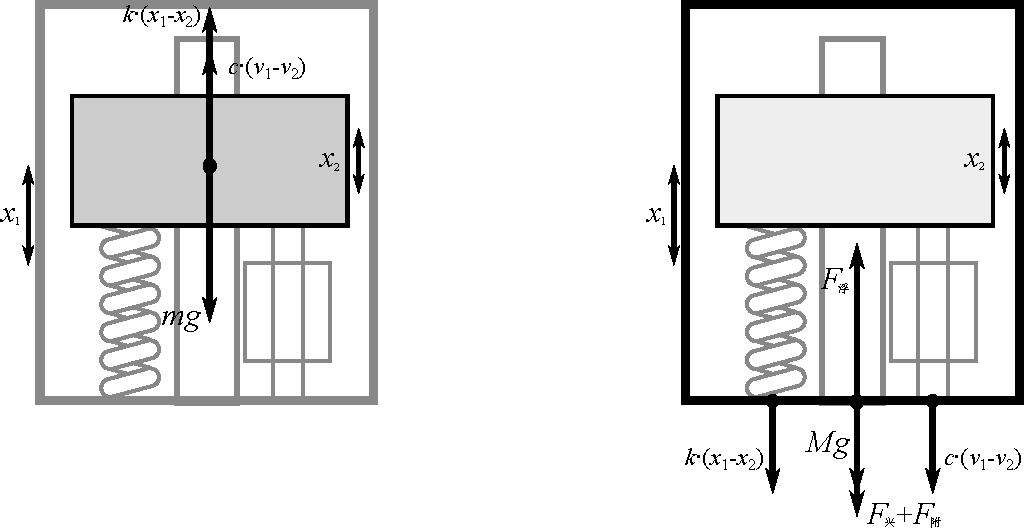
\includegraphics[width=11cm]{fig/force-analysis.pdf}
    \caption{对振子和浮子进行受力分析。为制图方便,未画出完整的浮子壳体}
    \label{force-analysis}
\end{figure}

我们需要确定起始时装置的深度。
记装置静止时受到的总浮力为 $F_\text{浮总}$,水的密度为 $\rho$,装置在水中漂浮时排水体积为 $V_\text{排总}$,则有
\begin{equation}
    \left\{
    \begin{aligned}
        & F_\text{浮总}=\rho gV_\text{排总} \\
        & (m+M)g=F_\text{浮总}
    \end{aligned}
    \right.
    \label{floating-relationship}
\end{equation}
代入附件 4 的数据容易求得 $V_\text{排总}\approx7.121\,\mathrm{m}^3$。
另一方面,考虑浮子下方锥体的体积,有 $V_\text{锥}=\dfrac{1}3\uppi r^2h\approx0.837\,\mathrm{m}^3$。显然,水没过了整个锥体部分,水面在浮子的柱体部分。此时,浮子因在液面中上升下降所造成的浮力变化 $\Delta F_\text{浮}=\rho g\Delta V_{排}=\rho gA\Delta x_1$,其中 $\Delta x_1$ 为浮子没入液面深度的变化量,$A$ 是圆柱的横截面面积。
从而有
\begin{equation}
    F_\text{浮}=F_\text{浮总}+\Delta F_\text{浮}=F_\text{浮总}-\rho gAx_1
    \label{floating}
\end{equation}

联立 \eqref{oscilator}—\eqref{floating} 式,我们可以消去 $mg$、$Mg$、$F_\text{浮}$ 和 $x_0$ 几项,得到
\begin{equation}
    \left\{
    \begin{aligned}
        &  m\dfrac{\dif^2x_2}{\dif t^2}=k(x_1-x_2)+c(\dfrac{\dif{x_1}}{\dif{t}}-\dfrac{\dif{x_2}}{\dif{t}}) \\
        &  M\dfrac{\dif^2x_1}{\dif t^2}=F-k(x_1-x_2)-c(\dfrac{\dif{x_1}}{\dif{t}}-\dfrac{\dif{x_2}}{\dif{t}})-\rho gAx_1-c_0\dfrac{\dif{x_1}}{\dif{t}}-m_0\dfrac{\dif^2 x_1}{\dif t^2}
    \end{aligned}
    \right.
    \label{chui-dang}
\end{equation}
式 \eqref{chui-dang} 就是关于浮子和振子垂荡运动的微分方程组。
考虑装置启动前静止,$t=0$ 时,有初值
\begin{equation}
    \left\{
    \begin{aligned}
        & x_1=x_2=0 \\
        & \dfrac{\dif x_1}{\dif t}=\dfrac{\dif x_2}{\dif t}=0
    \end{aligned}
    \right.
\end{equation}
求解这个初值问题,我们就能解出此题。

\subsubsection{问题求解}

根据附件 3 和附件 4,我们查得式 \eqref{chui-dang} 中的各个常数值如表 \ref{consts-1} 所示。
\begin{table}[htbp]
    \centering
    \begin{tabular}{cc}
        \toprule
        符号 & 常数的值 \\
        \midrule
        $M$ & \N{4866}\,kg \\
        $m$ & \N{2433}\,kg \\
        $k$ & \N{80000}\,$\mathrm{N}/\mathrm{m}$ \\
        $\rho$ & \N{1025}\,$\mathrm{kg}/\mathrm{m}^3$ \\
        $g$ & \N{9.8}\,$\mathrm{m}/\mathrm{s}^2$ \\
        $A$ & $\uppi\,\mathrm{m}^2$ \\
        $c_0$ & \N{656.3616}\,$\mathrm{N}\cdot\mathrm{s}/\mathrm{m}$ \\
        $m_0$ & \N{1335.535}\,kg \\
        \bottomrule
    \end{tabular}
    \caption{问题一适用的常量值}
    \label{consts-1}
\end{table}

同时,对于波浪激励力 $F$ 我们有
\begin{equation}
    F=f\cos(\omega t)
\end{equation}
其中 $f=\N{6250}\,\mathrm{N}$,$\omega=\N{1.4005}\,\mathrm{s}^{-1}$。
而对于阻尼系数 $c$,有
\begin{equation}
    c=\left\{
        \begin{aligned}
            & \N{10000}\,\mathrm{N}\cdot\mathrm{s}/\mathrm{m}, \text{对于情况 1} \\
            & \N{10000}\sqrt{\left|\dfrac{\dif x_1}{\dif t}-\dfrac{\dif x_2}{\dif t}\right|}\,\mathrm{N}\cdot(\mathrm{s}/\mathrm{m})^{3/2}, \text{对于情况 2}
        \end{aligned}
    \right.
\end{equation}

我们使用计算机对这个二元二阶线性初值问题进行数值求解。
对于题设的两种情况,我们均设定求解起点和终点为 0\,s 和 180\,s,以 0.2\,s 为间隔进行求解,得到在这 180\,s(即前 40 个周期)中,振子和浮子各自的位移和速度,如图所示。

完整的求解结果,我们已经存放在 \verb|result1-1.xlsx| 和 \verb|result1-2.xlsx| 文件中。其中,10\,s,20\,s,40\,s,60\,s,100\,s 时的数据如表 \ref{answer-1-1} 和表 \ref{answer-1-2} 所示。
\begin{table}[htbp]
    \centering
    \begin{tabular}{ccccccc}
        \toprule
        & & 10\,s & 20\,s & 40\,s & 60\,s & 100\,s \\
        \midrule
        \multirow{2}{*}{浮子} & 速度/$\mathrm{m}\cdot\mathrm{s}^{-1}$ & 1 & 2 & 3 & 4 & 5 \\
        & 位移/$\mathrm{m}$ & 1 & 2 & 3 & 4 & 5 \\
        \multirow{2}{*}{振子} & 速度/$\mathrm{m}\cdot\mathrm{s}^{-1}$ & 1 & 2 & 3 & 4 & 5 \\
        & 位移/$\mathrm{m}$ & 1 & 2 & 3 & 4 & 5 \\
        \bottomrule
    \end{tabular}
    \caption{当 $c$ 为定值时,求解得到几个特殊时刻的浮子、振子位移和速度数据}
    \label{answer-1-1}
\end{table}

\begin{table}[htbp]
    \centering
    \begin{tabular}{ccccccc}
        \toprule
        & & 10\,s & 20\,s & 40\,s & 60\,s & 100\,s \\
        \midrule
        \multirow{2}{*}{浮子} & 速度/$\mathrm{m}\cdot\mathrm{s}^{-1}$ & 1 & 2 & 3 & 4 & 5 \\
        & 位移/$\mathrm{m}$ & 1 & 2 & 3 & 4 & 5 \\
        \multirow{2}{*}{振子} & 速度/$\mathrm{m}\cdot\mathrm{s}^{-1}$ & 1 & 2 & 3 & 4 & 5 \\
        & 位移/$\mathrm{m}$ & 1 & 2 & 3 & 4 & 5 \\
        \bottomrule
    \end{tabular}
    \caption{当 $c$ 与相对速度相关时,求解得到几个特殊时刻的浮子、振子位移和速度数据}
    \label{answer-1-2}
\end{table}



\subsection{问题二}

\subsubsection{输出功率的推导}

波浪能系统的输出功率来自于 PTO 的阻尼力做功。
在 $t$ 时刻,设 PTO 的阻尼力为 $F_\text{PTO}$,记瞬时输出功率为 $P(t)$,则
    \begin{align}
        & F_\text{PTO}=c|v_1-v_2| \\
        & P(t)=F_\text{PTO}\Delta v=c(v_1-v_2)^2
    \end{align}
其中 $v_1$、$v_2$ 是浮子和振子的速度。
得到瞬时功率之后,将其在一段时间内累加(积分)并取平均值,即可得到平均输出功率
\begin{equation}
    \bar{P}=\dfrac{1}{T}\int\limits_0^TP(t)\dif t\approx\dfrac{1}{T}\sum_{i=1}^n\dfrac{P(t_i)+P(t_{i+1})}{2}\Delta t
\end{equation}
结合问题一的方法计算离散的速度、位移与时间的关系,我们容易算出给定条件下的 PTO 输出功率。

\subsubsection{最优参数的选择}

本题需要找出在 (1) $c$ 为常数且 $c\in[0, \N{100000}]\,(\mathrm{N}\cdot\mathrm{s}/\mathrm{m})$ 和 (2) $c=C|v_1-v_2|^p$,其中 $C\in[0, \N{100000}]\,(\mathrm{N}\cdot(\mathrm{s}/\mathrm{m})^{p+1})$ 和 $p\in[0, 1]$ 为常数的两种情况下,平均输出功率 $\bar{P}$ 的最大值和相应的常数系数。
本问题使用的与问题一所不同的量如表 \ref{consts-2} 所示。
\begin{table}[htbp]
    \centering
    \begin{tabular}{cc}
        \toprule
        符号 & 量的值 \\
        \midrule
        $F$ & $f\cos(\omega t)$,其中 $f=\N{4890}\,\mathrm{N}$,$\omega=\N{2.2143}\,\mathrm{s}^{-1}$ \\
        $c_0$ & $\N{167.8395}\,\mathrm{N}\cdot\mathrm{s}/\mathrm{m}$ \\
        $m_0$ & $\N{1165.992}\,\mathrm{kg}$ \\
        \bottomrule
    \end{tabular}
    \caption{问题二使用的与问题一不同的量}
    \label{consts-2}
\end{table}

对于传统的连续解析函数的极(最)值优化问题,我们有诸如爬山法、梯度下降法、Adams 算法等多种方法。
然而,这些方法都依赖函数的可导性质。
在问题一中,我们得到的是离散的点集,显然传统的函数优化方法不再适用。
为了高效地找到其中的最优化值,我们使用一种类似「随机梯度下降」的方法进行函数优化。


我们将上面的过程编写为 Python 程序并运行,最终运行得到的优化结果如表 \ref{answer-2-1} 和 \ref{answer-2-2} 所示。
\begin{table}[htbp]
    \centering
    \begin{tabular}{cc}
        \toprule
        输出功率/W & 阻尼系数/$\mathrm{N}\cdot\mathrm{s}/\mathrm{m}$ \\
        \midrule
        1 & 2 \\
        \bottomrule
    \end{tabular}
    \caption{输出功率的最大值,以及此时的阻尼系数}
    \label{answer-2-1}
\end{table}

\begin{table}[htbp]
    \centering
    \begin{tabular}{ccc}
        \toprule
        输出功率/W & 比例系数/$\mathrm{N}\cdot(\mathrm{s}/\mathrm{m})^{p+1}$ & 幂指数 \\
        \midrule
        1 & 2 & 3 \\
        \bottomrule
    \end{tabular}
    \caption{输出功率的最大值,以及此时的阻尼系数}
    \label{answer-2-2}
\end{table}

同时,为了直观验证结果的合理性,我们也使用 Wolfram Engine 内置的点集绘图功能,绘制了平均输出功率 $P$ 与阻尼系数、比例系数、幂指数等的关系图。
对于情况 1,关系如图 \ref{result-2-1} 所示,而对于情况 2,关系如图 \ref{result-2-2} 所示。
不难发现,我们使用算法得到的优化解,与图上所显示出的走向趋势一致。

\subsection{问题三}

\subsubsection{运动方程的建立}

与问题一相比,问题三加入了中轴的旋转,使得整个系统的运动变得复杂。
我们有必要建立新的细化的物理模型,从而列出新的运动方程。

本问题的模型中,外部浮子有两种不同类型的运动:一种是在竖直方向波浪激励力的作用下,在铅直方向进行的直线运动;另一种是在波浪激励力矩的影响下,绕某个轴进行的转动。
而在浮子的内部,振子由 PTO 和中轴所约束,PTO 和中轴的根部用一绞链与浮子相连结,亦绕绞链所在轴进行转动。
为了便于问题的分析,我们拟定下面的前提:
\begin{enumerate}
    \item 浮子的转动是绕其质心进行的定轴转动,振子的转动中心则是中轴与中轴底座绞接处。中轴底座、转轴等结构的厚度为零。
    \item 题目中所提供的波浪激励力矩 $L\cos(\omega t)$ 可视为力偶矩,它不为浮子的平动提供加速度。
\end{enumerate}

我们以整个装置静止直立在水面上时,浮子的质心为原点,以来流指向方向为 $x$ 轴正方向,以铅直向上为 $z$ 轴正方向,建立空间直角坐标系 $O-xyz$。
在装置运行的某一时刻 $t$,在 $xOz$ 投影面上装置的运行状态如图 \ref{status} 所示。
\begin{figure}[htbp]
    \centering
    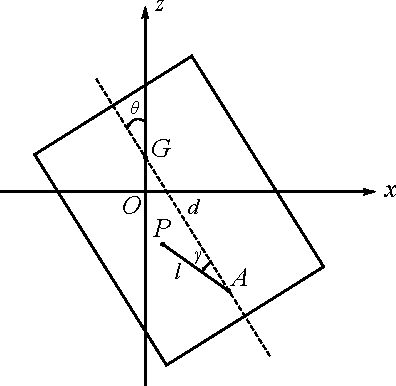
\includegraphics[width=6cm]{fig/problem-3-1.pdf}
    \caption{某时刻,$xOz$ 投影面上的装置运行状态}
    \label{status}
\end{figure}

在图中,$G$ 是浮子的质心。
显然,浮子是一个对称旋转体,故 $G$ 始终位于浮子的旋转轴(图中的虚线)上。
$A$ 点是绞链所在的点,由题目条件知道绞接处也位于浮子的旋转轴上。
$P$ 点是振子质心所在的点,$AP$ 连线表示的就是 PTO 和中轴构成的结构。
考虑装置中所有的转动,我们记 $\theta$ 为浮子的纵摇角,记 $\gamma$ 为振子相对于浮子的纵摇角,角度以图上视角逆时针为正值。
同时,为了便于分析,我们记 $l$ 为弹簧在此时的长度,记 $d$ 为线段 $AG$ 的长度,即转轴绞接处与浮子质心的距离。

方便起见,我们设此时 $G$ 点的坐标为 $(x_G, 0, z_G)$,设此时 $P$ 点的坐标为 $(x_P, 0, z_P)$。
对振子进行受力分析。
振子在水平和竖直方向产生的加速度分别为 $\dfrac{\dif^2 x_P}{\dif t^2}$ 和 $\dfrac{\dif^2 z_P}{\dif t^2}$,而振子受到的外力有 PTO 装置(弹簧和阻尼器)的推拉力 $F_\text{PTO}$、振子自身重力 $mg$ 以及其受到中轴(视为轻杆)的支持力 $F_{AB}$。
在 $x$ 和 $z$ 方向分别列出振子的运动学方程,有
\begin{align}
    m\cdot\dfrac{\dif^2 x_P}{\dif t^2} &= -F_\text{PTO}\sin(\theta+\gamma)+F_{AB}\cos(\theta+\gamma) \label{problem-3-eq1}\\
    m\cdot\dfrac{\dif^2 z_P}{\dif t^2} &= F_\text{PTO}\cos(\theta+\gamma)-mg+F_{AB}\sin(\theta+\gamma)
\end{align}

考虑振子的转动,设其在弹簧长度为 $l$ 时的转动惯量为 $I_B(l)$。
以逆时针为正方向。
记绞接处旋转阻尼器产生的旋转力矩为 $M_\text{PTO}$,则可以列出如下的转动运动学方程
\begin{equation}
    I_B(l)\cdot\dfrac{\dif^2(\theta+\gamma)}{\dif t^2}=M_\text{PTO}-F_{AB}\cdot l
\end{equation}

再来分析浮子。
% 在水平方向,由前文的前提分析可知,浮子受到的合力为零。
% 而在这一方向能产生分力的,只有 $F_{ABx}$ 和 $F_\text{PTO}$ 的反作用力。
% 我们容易得到
% \begin{equation}
%     F_\text{PTO}\sin(\theta+\gamma)-F_{ABx}=0
% \end{equation}
在水平方向,浮子只受到 $F_\text{PTO}$ 和 $F_{AB}$ 的水平分力,故有
\begin{equation}
    M\cdot\dfrac{\dif^2 x_G}{\dif t^2}= F_\text{PTO}\sin(\theta+\gamma)-F_{AB}\cos(\theta+\gamma)
\end{equation}
而在竖直方向,浮子受到波浪激励力 $F$、自身重力 $Mg$、PTO 反作用力 $F_\text{PTO}$ 的竖直分力、杆支持力的反作用力 $F_{AB}$ 的水平竖直分力,以及浮力(静水恢复力) $F_\text{浮}$、附加惯性力 $m_0\dfrac{\dif^2z_G}{\dif t^2}$、兴波阻尼力 $c_0\dfrac{\dif z_G}{\dif t}$。
因此有
\begin{equation}
    M\cdot\dfrac{\dif^2 z_G}{\dif t^2}=F+F_\text{浮}-Mg-F_\text{PTO}\cos(\theta+\gamma)-F_{AB}\sin(\theta+\gamma)-m_0\dfrac{\dif^2z_G}{\dif t^2}-c_0\dfrac{\dif z_G}{\dif t}
\end{equation}

最后,我们分析浮子的转动过程。
记波浪激励力矩为 $M_\text{wave}$,浮子绕过其质心的轴的转动惯量为 $I_A$,附加转动惯量为 $I_0$,兴波阻尼力矩系数为 $c_\text{r0}$,静水恢复力矩系数为 $M_\text{rec}$,有
\begin{equation}
    I_A\dfrac{\dif^2\theta}{\dif t^2}=M_\text{wave}-M_\text{PTO}-F_{AB}\cos(\theta+\gamma)\cdot d\cos\theta-F_{AB}\sin(\theta+\gamma)\cdot d\sin\theta-I_0\dfrac{\dif^2\theta}{\dif t^2}-c_\text{r0}\dfrac{\dif\theta}{\dif t}-M_\text{rec}\theta \label{problem-3-eq5}
\end{equation}

式 \eqref{problem-3-eq1}—\eqref{problem-3-eq5} 构成一组微分方程组。
其中的未知函数是 $\theta$、$\gamma$、$l$、$z_G$、$x_G$ 和 $F_{AB}$,它们都是时间 $t$ 的函数。
下面,我们尝试确定上述方程中的系数和常数,从而使得微分方程可以被解算。

\subsubsection{参数的求值}

考虑弹簧和阻尼器构成的 PTO。
容易知道
\begin{equation}
    F_\text{PTO}=-k(l-l_0)-c\dfrac{\dif l}{\dif t}
\end{equation}

考虑转轴绞接处的旋转 PTO,记扭转弹簧的刚度系数为 $k_\text{rot}$,旋转阻尼器的阻尼系数为 $c_\text{rot}$,有
\begin{equation}
    M_\text{PTO}=-k_\text{rot}\gamma-c_\text{rot}\dfrac{\dif \gamma}{\dif t}
\end{equation}

考虑几何关系,有
\begin{align}
    x_P&=x_G+d\sin\theta-l\sin(\theta+\gamma) \\
    z_P&=z_G-d\cos\theta+l\cos(\theta+\gamma)
\end{align}

考虑浮子的质心 $G$。
显然浮子是由一个无底圆锥面、一个圆柱侧面和一个圆面构成的组合体,对此组合体的各个部分求质心,我们容易求得此组合体的质心距离圆锥部分顶点的长度为 $d_G\approx\N{2.20792}\,\mathrm{m}$。
故 $d=d_G-\N{0.8}\,\mathrm{m}=\N{1.40792}\,\mathrm{m}$。

考虑浮子在做摇荡运动时的的排水量变化。
如图 \ref{floating-fig} 所示,设原先质心位置为 $G_0$,现在质心位置为 $G$,浮子角度为 $\theta$。
为了计算当前浮子排水的体积,我们可以延长 $GG_0$ 和 $AG$ 到海平面,容易知道 $BG=\dfrac{d_G}{\cos\theta}$。
因此 $AB=AG+GB$ 可以容易算出。
另一方面,由对称性可知 $V_A=V_B$,因此排水体积即为 $B$ 点之下浮子的体积。
代入数据得
\begin{equation}
    V_\text{排}=\N{5.2609}+\N{1.86007}\sec \theta-\uppi z_G\sec \theta
\end{equation}

\begin{figure}[htbp]
    \centering
    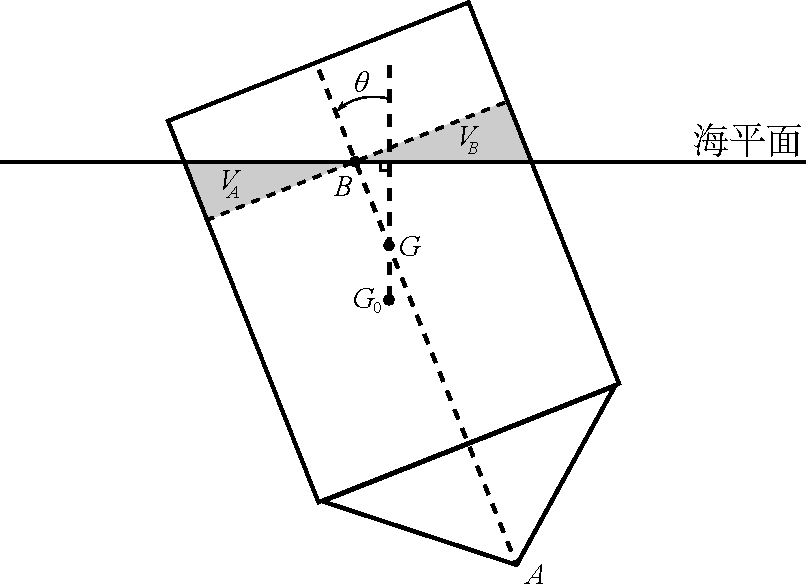
\includegraphics[width=8cm]{fig/floating.pdf}
    \caption{浮子排水量计算示意}
    \label{floating-fig}
\end{figure}

考虑浮子绕重心做纵摇运动的转动惯量,易知该浮子可以看成是由一个无底圆锥面、一个圆柱侧面和一个圆面的组合体。
容易知道
\begin{equation}
    I_A=I_\text{锥}+I_\text{柱}+I_\text{圆}
\end{equation}
我们先考虑一个理想均匀细圆环绕一平行于其直径的转轴旋转时的转动惯量。
记圆环半径为 $R$,转轴到圆环所在平面距离为 $l$。
取圆环上 $\dif\theta$ 角对应的一小段,其长度为 $R\dif\theta$。
若圆环线密度为 $\lambda$,则这段圆环的转动惯量
\begin{equation}
    \dif I=\lambda\cdot R\dif\theta(l^2+R^2\cos^2\theta)
\end{equation}
所以对整个环有
\begin{equation}
    I_\text{ring}=\int\limits_0^{2\uppi}\lambda R\dif\theta(l^2+R^2\cos^2\theta)
\end{equation}
圆锥面、圆柱面和圆盘都可以分解为圆环在特定方向上的积分。
对圆锥,记半顶角大小为 $\delta$,有
\begin{equation}
    \begin{aligned}
        I_\text{锥} &= \int\limits_0^{h_\text{锥}}I_\text{ring}\dif p \\
        &=\int\limits_0^{h_\text{锥}}\dfrac{1}{\cos\delta}\dif p\int\limits_0^{2\uppi}\rho p\tan\delta((\d_G-p)^2+(p\tan\delta)^2\cos^2\theta)\dif\theta
    \end{aligned}
\end{equation}
同理对圆柱有
\begin{equation}
        I_\text{柱} = \int\limits_{h_\text{柱底}}^{h_\text{柱顶}}\dif p\int\limits_{0}^{2\uppi}\rho R(p^2+R^2\cos^2\theta)\dif\theta
\end{equation}
对圆面有
\begin{equation}
    I_\text{圆} = \int\limits_0^R\dif p\int\limits_0^{2\uppi}\rho p(l^2+p^2\cos^2\theta)\dif\theta
\end{equation}
我们代入相应的尺寸数据,得到
\begin{equation}
    I_A=\N{8399.2}\,\mathrm{kg}\cdot\mathrm{m}^2
\end{equation}

另一方面,我们考虑振子绕转轴转动的转动惯量,有转轴绞接处到振子底部圆心的距离为 $l$。
设振子圆柱体厚度为 $h$,半径为 $r$,有
\begin{equation}
        I_B(l) =\dfrac{(4h^2-12h(h+l)+3r^2+12(h+l)^2)m}{12} 
        \label{last-eq-3}
\end{equation}    

联立式 \eqref{problem-3-eq1}—\eqref{last-eq-3},可以得到一组有六个未知函数的微分方程。

\subsubsection{数值求解}

对于问题三,我们使用的常量如表 \ref{consts-3} 所示。

\begin{table}[htbp]
    \centering
        \begin{tabular}{cc}
            \toprule
            符号 & 常数的值 \\
            \midrule
            $M$ & \N{4866}\,kg \\
            $m$ & \N{2433}\,kg \\
            $\rho$ & \N{1025}\,$\mathrm{kg}/\mathrm{m}^3$ \\
            $g$ & \N{9.8}\,$\mathrm{m}/\mathrm{s}^2$ \\
            $A$ & $\uppi\,\mathrm{m}^2$ \\
            $k$ & \N{8000}\,$\mathrm{N}/\mathrm{m}$ \\
            $c$ & $\N{10000}\,\mathrm{N}\cdot\mathrm{s}/\mathrm{m}$ \\
            $k_\text{rot}$ & $\N{250000}\,\mathrm{N}\cdot\mathrm{m}$ \\
            $c_\text{rot}$ & $\N{1000}\,\mathrm{N}\cdot\mathrm{m}\cdot\mathrm{s}$ \\
            $l_0$ & $\N{0.5}\,\mathrm{m}$ \\
            $M_\text{rec}$ & $\N{8890.7}\,\mathrm{N}\cdot\mathrm{m}$ \\
            $m_0$ & $\N{1028.876}\,\mathrm{kg}$ \\
            $I_0$ & $\N{7001.914}\,\mathrm{kg}\cdot\mathrm{m}^2$ \\
            $c_0$ & $\N{683.4558}\,\mathrm{N}\cdot\mathrm{s}/\mathrm{m}$ \\
            $c_\text{r0}$ & $\N{655.3383}\,\mathrm{N}\cdot\mathrm{m}\cdot\mathrm{s}$ \\
            \bottomrule
        \end{tabular}    
        \caption{问题三适用的常量值}
        \label{consts-3}
\end{table}        

同时,本问题中使用的波浪激励力和力矩 $F$ 与 $M_\text{wave}$ 满足
\begin{equation*}
    \left\{
    \begin{aligned}
        & F=f\cos(\omega t) \\
        & M_\text{wave}=L\cos(\omega t) \\
        & f=\N{3640}\,\mathrm{N} \\
        & L=\N{1690}\,\mathrm{N}\cdot\mathrm{m} \\
        & \omega=\N{1.7152}\,\mathrm{s}^{-1} \\
    \end{aligned}    
    \right.
\end{equation*}    

将以上方程输入计算机中求解,可以得到各个时刻下浮子和振子的位移、速度、角位移、角速度,如图至图所示。
完整的求解结果,我们已经存放在 \verb|result3.xlsx|文件中。其中,10 s,20 s,40 s,60 s,100 s 时的数据如表 和表 所示。

\subsection{问题四}

\subsubsection{输出功率的推导}

问题四在问题二的基础上,增加了绕轴旋转的纵摇运动。
我们可以利用问题三已经计算出来的各个时刻的浮子、振子状态,来计算一系列瞬时功率并进行积分,即可求得平均功率。



    \section{模型检验与评价}

模型者,好也。
    \newpage
\printbibliography[heading=bibintoc]
    %% APPENDIX
    \appendix
    \newpage
\section{程序源代码}

\subsection{Wolfram 程序源代码}

我们使用 Wolframe 语言编写了求解问题一至问题四的程序。
它们的源代码如下。
若要运行这些代码,请使用 Mathematica 13 或对应版本的 Wolfram Engine for Developers 软件输入下面的代码并运行。

此处的代码即是 \verb|final.nb| 文件中的输入命令集合。

\begin{lstlisting}[language=Mathematica,breaklines]
Clear["Global`*"];
问题 1
第 1 小问
m=2433;k=80000;c=10000;
f=6250;omega=1.4005;k1=1025*9.8*Pi;
c0=656.3616;m0=1335.535;M=4866;
stop=40/omega*2*Pi;
s=NDSolve[{m*x2''[t]==k(x1[t]-x2[t])+c(x1'[t]-x2'[t]),f*Cos[omega*t]==k(x1[t]-x2[t])+c(x1'[t]-x2'[t])+k1*x1[t]+c0*x1'[t]+m0*x1''[t]+M*x1''[t],x1[0]==x2[0]==x1'[0]==x2'[0]==0},{x1,x2},{t,0,Max[stop,100]}];
Plot[Evaluate[{x1[t],x2[t]}/.s],{t,0,Min[stop,100]},PlotLegends->Placed[{"x1","x2"},{1,0.5}],PlotStyle->{Directive[Blue,Thick],Directive[Orange,Dashed]}]
Plot[Evaluate[{x1[t]-x2[t],x1'[t]-x2'[t]}/.s],{t,0,Min[stop,100]},PlotLegends->Placed[{"\[CapitalDelta]x","\[CapitalDelta]v"},{1,0.5}]]

targets={10,20,40,60,100};
data=Table[{i,First[x1[i]/.s],First[x1'[i]/.s],First[x2[i]/.s],First[x2'[i]/.s]},{i,targets}];
Grid[data,Frame->All]
Export["~/cumcm/cumcm-code/P11-paper.xlsx",data]

Export["~/cumcm/cumcm-code/P11.xlsx",Flatten[Table[{i,x1[i],x1'[i],x2[i],x2'[i]}/.s,{i,Range[0,40/omega*2*Pi,0.2]}],1]]

第 (2) 小问
cv2[v_]:=10000*Sqrt[Abs[v]]
s=NDSolve[{m*x2''[t]==k(x1[t]-x2[t])+cv2[x2'[t]]*(x1'[t]-x2'[t]),f*Cos[omega*t]==k(x1[t]-x2[t])+cv2[x2'[t]]*(x1'[t]-x2'[t])+k1*x1[t]+c0*x1'[t]+m0*x1''[t]+M*x1''[t],x1[0]==x2[0]==x1'[0]==x2'[0]==0},{x1,x2},{t,0,Max[stop,100]}];
Plot[Evaluate[{x1[t],x2[t]}/.s],{t,0,Min[stop,100]},PlotLegends->Placed[{"x1","x2"},{1,0.5}],PlotStyle->{Directive[Green,Thick],Directive[Pink,Dashed]}]

targets={10,20,40,60,100};
data=Table[{i,First[x1[i]/.s],First[x1'[i]/.s],First[x2[i]/.s],First[x2'[i]/.s]},{i,targets}];
Grid[data,Frame->All]

Export["~/cumcm/cumcm-code/P12-paper.xlsx",data]
Plot[Evaluate[{x1[t]-x2[t],x1'[t]-x2'[t]}/.s],{t,0,Min[stop,100]},PlotLegends->Placed[{"\[CapitalDelta]x","\[CapitalDelta]v"},{1,0.5}]]
Export["~/cumcm/cumcm-code/P12.xlsx",Flatten[Table[{i,x1[i],x1'[i],x2[i],x2'[i]}/.s,{i,Range[0,40/omega*2*Pi,0.2]}],1]]

第 2 题
第 (1) 小问
Clear["Global`*"];
M=4866;m=2433;k=80000;c=10000;omega=2.2143;k1=1025*9.8*Pi;
f=4890;c0=167.8395;m0=1165.992;
start=110;stop=start+20*1/omega*2*Pi;dim=0.01;
P21[cm2_]:=(Sum[cm2*((x1'[i]-x2'[i])^2)*dim,{i,start,stop,dim}]/.NDSolve[{m*x2''[t]==k*(x1[t]-x2[t])+cm2*(x1'[t]-x2'[t]),f*Cos[omega*t]==k*(x1[t]-x2[t])+cm2*(x1'[t]-x2'[t])+k1*x1[t]+c0*x1'[t]+m0*x1''[t]+M*x1''[t],x1[0]==x2[0]==x1'[0]==x2'[0]==0},{x1,x2},{t,start,stop}])/(stop-start)
DrawP21[pStart_,pStop_,pStepNum_,name_]:=ListLinePlot[Table[{i,First[P21[i]]},{i,Range[pStart,pStop,(pStop-pStart)/pStepNum]}],PlotLegends->Placed[name,{1,0.5}]]
DrawP21[0,100000,100,"P(c)"]
DrawP21[37250,37270,100,"P(c)"]

第 (2) 小问
Clear["Global`*"];
M=4866;m=2433;k=80000;c=10000;omega=2.2143;k1=1025*9.8*Pi;
f=4890;c0=167.8395;m0=1165.992;
start=110;stop=start+20*1/omega*2*Pi;dim=0.01;
cmv2[v_,ck_,ce_]:=ck*Abs[v]^ce;
P22I[ck_,ce_]:=NDSolve[{m*x2''[t]==k*(x1[t]-x2[t])+cmv2[x1'[t]-x2'[t],ck,ce]*(x1'[t]-x2'[t]),f*Cos[omega*t]==k*(x1[t]-x2[t])+cmv2[x1'[t]-x2'[t],ck,ce]*(x1'[t]-x2'[t])+k1*x1[t]+c0*x1'[t]+m0*x1''[t]+M*x1''[t],x1[0]==x2[0]==x1'[0]==x2'[0]==0},{x1,x2},{t,start,stop}]
P22[ck_,ce_]:=(Sum[cmv2[x1'[i]-x2'[i],ck,ce+2]*dim,{i,start,stop,dim}]/.P22I[ck,ce])/(stop-start)
CalcP22[kStart_,kStop_,kStepNum_,eStart_,eStop_,eStepNum_]:=Parallelize[Table[{pe,ppk,First[P22[ppk,pe]]},{ppk,Range[kStart,kStop,(kStop-kStart)/kStepNum]},{pe,Range[eStart,eStop,(eStop-eStart)/eStepNum]}]]
DrawP22[data_]:=ListPlot3D[Flatten[data,1]]
s=CalcP22[0,100000,8,0,1,8];
ss=Table[{i[[1]],i[[2]]/10000,i[[3]]},{i,Flatten[s,1]}];
(*Grid[N[s],Frame->All]*)
ListPlot3D[ss]
ListContourPlot[ss]
(*ListDensityPlot[ss]*)

第 3 题
Clear["Global`*"];
(*AG长度*)
d=1.40792;
(*弹簧原长度*)
l0=0.5;
(*振子质量*)
m=2433;
(*弹簧劲度系数*)
k=80000;
(*直线阻尼器阻尼系数*)
c=10000;
(*小g*)
g=9.8;
(*弹簧旋转刚度*)
krot=250000;
(*旋转阻尼器阻尼系数*)
crot=1000;
(*浮子质量*)
M=4866;
(*垂荡兴波阻尼系数*)
c0=683.4558;
(*纵摇附加转动惯量*)
I0=7001.914;
(*纵摇激励力矩振幅*)
L=1690;
(*入射波浪频率*)
w=1.7152;
(*垂荡激励力振幅*)
f=3640;
(*浮子转动惯量*)
Ia=8399.2;

(*垂荡附加质量*)
m0=1028.876;
(*纵摇兴波阻尼力矩系数*)
cr0=654.3383;
(*纵摇静水恢复力矩系数*)
Mrec=8890.7;
(*海水密度*)
rho=1025;

(*垂荡静水恢复力(浮力)*)
Fj[t_]:=(5.2609+1.86007*Sec[th[t]]-Pi*zg[t]*Sec[th[t]])*rho*g;
(*激励力*)
Fwave[t_]:=f*Cos[w*t];
(*振子转动惯量*)
Ib[t_]:=m/12*(4*0.5^2-12*0.5*(0.5+l[t])+3*1^2+12*(0.5+l[t])^2)
(*纵摇激励力矩*)
Mwave[t_]:=L*Cos[w*t];
(*theta2=theta1+gamma*)
th2[t_]:=th[t]+ga[t];
(*P点x座标*)
xp[t_]:=d*Sin[th[t]]-l[t]*Sin[th2[t]];
(*P点z座标*)
zp[t_]:=zg[t]-d*Cos[th[t]]+l[t]*Cos[th2[t]];
(*PTO系统的力*)
Fpto[t_]:=-k*(l[t]-l0)-c*l'[t];
(*PTO系统的力矩*)
Mpto[t_]:=-krot*ga[t]-crot*ga'[t];

start=0;
stop=start+40/w*2*Pi;
group={m*xp''[t]==-Fpto[t]*Sin[th2[t]]+Fab[t]*Cos[th2[t]],m*zp''[t]==Fpto[t]*Cos[th2[t]]-m*g+Fab[t]*Sin[th2[t]],Ib[t]*th2''[t]==Mpto[t]+Fab[t]*l[t],M*zg''[t]==Fwave[t]+Fj[t]-M*g-Fpto[t]*Cos[th2[t]]-Fab[t]*Sin[th2[t]]-m0*zg''[t]-c0*zg'[t],Ia*th''[t]==Mwave[t]-Mpto[t]+Fab[t]*d*Cos[th[t]]*Cos[th2[t]]-Fab[t]*d*Sin[th[t]]*Sin[th2[t]]-I0*th''[t]-cr0*th'[t]-Mrec*th[t],th'[0]==th[0]==ga[0]==ga'[0]==l'[0]==zg'[0]==0,l[0]==l0-m/k,zg[0]==0};
s=NDSolve[group,{th,ga,zg,l},{t,start,Max[stop,100]}];
Plot[{th[t]/.s,ga[t]/.s},{t,start,Min[stop,100]},PlotLegends->Placed[{"\[Theta]","\[Gamma]"},{1,0.5}]]
Plot[{th'[t]/.s,ga'[t]/.s},{t,start,Min[stop,100]},PlotLegends->Placed[{"\[Theta]'","\[Gamma]'"},{1,0.5}]]
Plot[{l[t]/.s,zg[t]/.s},{t,start,Min[stop,100]},PlotLegends->Placed[{"l","Zg"},{1,0.5}]]
Plot[{l'[t]/.s,zg'[t]/.s},{t,start,Min[stop,100]},PlotLegends->Placed[{"l'","Zg'"},{1,0.5}]]
(*Plot[Fj[t]/.s,{t,0,stop},PlotLegends->{"F浮"}]*)

targets={10,20,40,60,100};
data=Table[{t,First[zg[t]/.s],First[zg'[t]/.s],First[th[t]/.s],First[th'[t]/.s],First[l[t]/.s],First[l'[t]/.s],First[ga[t]/.s],First[ga'[t]/.s]},{t,targets}];
Grid[data,Frame->All]
Export["~/cumcm/cumcm-code/P3-paper.xlsx",data]

dl[t_]:=l[t]-l0
data=Table[{t,First[ff[t]/.s]},{ff,{zg,zg',th,th',dl,l',ga,ga'}},{t,0,40/w*2*Pi,0.2}];
save=Table[{t,First[zg[t]/.s],First[zg'[t]/.s],First[th[t]/.s],First[th'[t]/.s],First[dl[t]/.s],First[l'[t]/.s],First[ga[t]/.s],First[ga'[t]/.s]},{t,0,40/w,0.2}];
ListLinePlot[data,PlotLegends->{Zg,Zg',theta,theta',dl,l',gamma,gamma'}]
Export["~/cumcm/cumcm-code/P3.xlsx",save]

第4题
Clear["Global`*"];
(*AG长度*)
d=1.40792;
(*弹簧原长度*)
l0=0.5;
(*振子质量*)
m=2433;
(*弹簧劲度系数*)
k=80000;
(*小g*)
g=9.8;
(*弹簧旋转刚度*)
krot=250000;
(*浮子质量*)
M=4866;
(*垂荡兴波阻尼系数*)
c0=528.5018;
(*纵摇附加转动惯量*)
I0=7142.493;
(*纵摇激励力矩振幅*)
L=2140;
(*入射波浪频率*)
w=1.9806;
(*垂荡激励力振幅*)
f=1760;
(*浮子转动惯量*)
Ia=8399.2;

(*垂荡附加质量*)
m0=1091.099;
(*纵摇兴波阻尼力矩系数*)
cr0=1655.909;
(*纵摇静水恢复力矩系数*)
Mrec=8890.7;
(*海水密度*)
rho=1025;

(*垂荡静水恢复力(浮力)*)
Fj[t_]:=(5.2609+1.86007*Sec[th[t]]-Pi*zg[t]*Sec[th[t]])*rho*g;
(*激励力*)
Fwave[t_]:=f*Cos[w*t];
(*振子转动惯量*)
(*Ib[t_]:=258.149+774.448l[t]+1548.9l[t]^2;*)
(*Ib[t_]:=MomentOfInertia[Cylinder[{{0,0,0},{0.5,0,0}},0.5],{l[t]+0.5,0,0},{0,0,1}]*)
Ib[t_]:=m/12*(4*0.5^2-12*0.5*(0.5+l[t])+3*1^2+12*(0.5+l[t])^2)
(*纵摇激励力矩*)
Mwave[t_]:=L*Cos[w*t];
(*theta2=theta1+gamma*)
th2[t_]:=th[t]+ga[t];
(*P点x座标*)
xp[t_]:=d*Sin[th[t]]-l[t]*Sin[th2[t]];
(*P点z座标*)
zp[t_]:=zg[t]-d*Cos[th[t]]+l[t]*Cos[th2[t]];
(*PTO系统的力*)
Fpto[t_,c_]:=-k*(l[t]-l0)-c*l'[t];
(*PTO系统的力矩*)
Mpto[t_,crot_]:=-krot*ga[t]-crot*ga'[t];

start=100;
stop=start+5/w*2*Pi;
dim=0.2;
P4[c_,crot_]:=((Sum[(c*(l'[t]^2)+crot*(ga'[t]^2))*dim,{t,start,stop,dim}]/.NDSolve[{m*xp''[t]==-Fpto[t,c]*Sin[th2[t]]+Fab[t]*Cos[th2[t]],m*zp''[t]==Fpto[t,c]*Cos[th2[t]]-m*g+Fab[t]*Sin[th2[t]],Ib[t]*th2''[t]==Mpto[t,crot]+Fab[t]*l[t],M*zg''[t]==Fwave[t]+Fj[t]-M*g-Fpto[t,c]*Cos[th2[t]]-Fab[t]*Sin[th2[t]]-m0*zg''[t]-c0*zg'[t],Ia*th''[t]==Mwave[t]-Mpto[t,crot]+Fab[t]*d*Cos[th[t]]*Cos[th2[t]]-Fab[t]*d*Sin[th[t]]*Sin[th2[t]]-I0*th''[t]-cr0*th'[t]-Mrec*th[t],th'[0]==th[0]==ga[0]==ga'[0]==l'[0]==zg'[0]==0,l[0]==l0-m/k,zg[0]==0},{th,ga,zg,l},{t,start,stop}])/(stop-start))
CalcP4[kStart_,kStop_,kStepNum_,eStart_,eStop_,eStepNum_]:=Parallelize[Table[{pe,ppk,First[P4[ppk,pe]]},{ppk,Range[kStart,kStop,(kStop-kStart)/kStepNum]},{pe,Range[eStart,eStop,(eStop-eStart)/eStepNum]}]]
s=CalcP4[0,100000,8,0,100000,8];

(*Grid[N[s],Frame->All]*)
ss=Flatten[s,1];
ListPlot3D[ss]
ListContourPlot[ss]
ListContourPlot[ss,PlotRange->{740,960}]    
\end{lstlisting}

\subsection{Python 程序源代码}

我们使用 Python 语言编写了求解问题二和问题四的程序。
它们的源代码如下。
若要运行这些代码,请使用 Python 3.10.4 及以上的 Python 运行程序。
此外,可能需要安装一些额外的 Python 模块。

此处的源代码即是支撑材料中的 \verb|P24.py| 文件。

\begin{lstlisting}[language=Python,breaklines=true]
import sys
import threading
import queue
import time
from wolframclient.evaluation import WolframLanguageSession
from wolframclient.language import wl, wlexpr
import matplotlib.pyplot as plt
import random
import math
from functools import reduce
# import nest_asyncio
# nest_asyncio.apply()
# from wolframclient.evaluation import parallel_evaluate

P21 = """
Clear["Global`*"];
M = 4866; m = 2433; k = 80000; c = 10000; omega = 2.2143; k1 = 1025 * 9.8 * Pi;
f = 4890; c0 = 167.8395; m0 = 1165.992;
start = 110; stop = start + 20 * 1 / omega*2*Pi; dim = 0.01;
P21[cm2_] := (Sum[cm2 * ((x1'[i] - x2'[i])^2) * dim, {i, start, stop, dim}] /. 
  NDSolve[{m*x2''[t]==k*(x1[t]-x2[t])+cm2*(x1'[t]-x2'[t]), 
    f*Cos[omega * t]==k*(x1[t]-x2[t])+cm2*(x1'[t]-x2'[t])+k1*x1[t]+c0*x1'[t]+m0*x1''[t]+M*x1''[t], 
    x1[0]==x2[0]==x1'[0]==x2'[0]==0},
  {x1, x2}, {t, start, stop}]) / (stop-start)
"""

P22 = """
Clear["Global`*"];
M = 4866; m = 2433; k = 80000; c = 10000; omega = 2.2143; k1 = 1025 * 9.8 * Pi;
f = 4890; c0 = 167.8395; m0 = 1165.992;
start = 110; stop = start + 20 * 1 / omega*2*Pi; dim = 0.01;
cmv2[v_, ck_, ce_] := ck * Abs[v]^ce;
P22I[ck_, ce_] := NDSolve[{m*x2''[t]==k*(x1[t]-x2[t])+cmv2[x1'[t]-x2'[t], ck, ce]*(x1'[t]-x2'[t]), 
    f*Cos[omega * t]==k*(x1[t]-x2[t])+cmv2[x1'[t]-x2'[t], ck, ce]*(x1'[t]-x2'[t])+k1*x1[t]+c0*x1'[t]+m0*x1''[t]+M*x1''[t], 
    x1[0]==x2[0]==x1'[0]==x2'[0]==0},
  {x1, x2}, {t, start, stop}]
P22[ck_, ce_] := (Sum[cmv2[x1'[i]-x2'[i], ck, ce+2] * dim, {i, start, stop, dim}] /. P22I[ck, ce]) / (stop-start)
"""

P4 = '''
Clear["Global`*"];
(* AG长度 *)
d = 1.40792;
(* 弹簧原长度 *)
l0 = 0.5; 
(* 振子质量 *)
m = 2433; 
(* 弹簧劲度系数 *)
k = 80000;
(* 小g *)
g = 9.8;
(* 弹簧旋转刚度 *)
krot = 250000;
(* 浮子质量 *)
M = 4866;
(* 垂荡兴波阻尼系数 *)
c0 = 528.5018;
(* 纵摇附加转动惯量 *)
I0 = 7142.493;
(* 纵摇激励力矩振幅 *)
L = 2140;
(* 入射波浪频率 *)
w = 1.9806;
(* 垂荡激励力振幅 *)
f = 1760;
(* 浮子转动惯量 *)
(* Ia = 300*4866/(7 \[Pi]+(Sqrt[41] \[Pi])/5)*(Integrate[1/0.8*2*Pi*(r+(17.6+8/75*(Sqrt[41]))/(7+(Sqrt[41])/5))*r^2,{r,-(17.6+8/75*(Sqrt[41]))/(7+(Sqrt[41])/5),-(17.6+8/75*(Sqrt[41]))/(7+(Sqrt[41])/5)+0.8}]+Integrate[2*Pi*r^2,{r,-(17.6+8/75*(Sqrt[41]))/(7+(Sqrt[41])/5)+0.8,-(17.6+8/75*(Sqrt[41]))/(7+(Sqrt[41])/5)+3.8}]+Integrate[2*Pi*(3.8-(17.6+8/75*(Sqrt[41]))/(7+(Sqrt[41])/5))^2+a^2,{a,0,0.5}]); *)
Ia = 8399.2;

(* 垂荡附加质量 *)
m0 = 1091.099;
(* 纵摇兴波阻尼力矩系数 *)
cr0 = 1655.909;
(* 纵摇静水恢复力矩系数 *)
Mrec = 8890.7;
(* 海水密度 *)
rho = 1025;

(* 垂荡静水恢复力(浮力) *)
Fj[t_] := (7.120975609756098 - Pi*zg[t]) * rho * g;
(* 激励力 *)
Fwave[t_] := f * Cos[w*t];
(* 振子转动惯量 *)
(* Ib[t_] := 258.149 + 774.448 l[t] + 1548.9 l[t]^2; *)
(* Ib[t_] := MomentOfInertia[Cylinder[{{0, 0, 0}, {0.5, 0, 0}}, 0.5], {l[t] + 0.5, 0, 0}, {0, 0, 1}] *)
Ib[t_] := m / 12 * (4*0.5^2-12*0.5*(0.5+l[t])+3*1^2+12*(0.5+l[t])^2)
(* 纵摇激励力矩 *)
Mwave[t_] := L * Cos[w*t];
(* theta2 = theta1 + gamma *)
th2[t_] := th[t] + ga[t]; 
(* P点x座标 *)
xp[t_] := d*Sin[th[t]] - l[t]*Sin[th2[t]]; 
(* P点z座标 *)
zp[t_] := zg[t] - d*Cos[th[t]] + l[t]*Cos[th2[t]]; 
(* PTO系统的力 *)
Fpto[t_, c_] := -k*(l[t] - l0) - c*l'[t];
(* PTO系统的力矩 *)
Mpto[t_, crot_] := -krot*ga[t] - crot*ga'[t];

start = 100;
stop = start + 5 / w * 2 * Pi;
dim = 0.2;

P4[c_, crot_] := ((Sum[(c * (l'[t]^2) + crot * (ga'[t]^2)) * dim, {t, start, stop, dim}] /. NDSolve[{
    m*xp''[t] == -Fpto[t,c]*Sin[th2[t]] + Fab[t]*Cos[th2[t]], 
    m*zp''[t] == Fpto[t,c]*Cos[th2[t]] - m*g + Fab[t]*Sin[th2[t]], 
    Ib[t]*th2''[t] == Mpto[t,crot] + Fab[t]*l[t],
    M*zg''[t] == Fwave[t] + Fj[t] - M*g - Fpto[t,c]*Cos[th2[t]] - Fab[t]*Sin[th2[t]] - m0*zg''[t] - c0*zg'[t],
    Ia*th''[t] == Mwave[t] - Mpto[t,crot] + Fab[t]*d*Cos[th[t]]*Cos[th2[t]] - Fab[t]*d*Sin[th[t]]*Sin[th2[t]] - I0*th''[t] - cr0*th'[t] - Mrec*th[t],
    th'[0] == th[0] == ga[0] == ga'[0] == l'[0] == zg'[0] == 0, l[0] == l0-m/k, zg[0] == 0}, {th, ga, zg, l}, {t, start, stop}]) / (stop - start))'''

queue_task = queue.Queue()
queue_res = queue.Queue()

random.seed(11451419198)
tot = 0
threads = []
thread_num = 16
thread_running = False
thread_cmd_name = "P22"
thread_command = P22

# use_parallelize = True
use_parallelize = False

def thread_run(command, name):
    # print("thread start:", threading.current_thread())
    session = WolframLanguageSession()
    session.evaluate(command)
    # print("test exec:", session.evaluate(wlexpr("P22[90000, 0.4]")))
    while True:
        try:
            try:
                task = queue_task.get(block=True, timeout=1)
                if task is None:
                    break
                # print("got", task)
                if thread_cmd_name == "P21":
                    text = f"First[{name}[{task[0]}]]"
                else:
                    text = f"First[{name}[{task[0]}, {task[1]}]]"
                try:
                    res = session.evaluate(wlexpr(text))
                    if not isinstance(res, float):
                        raise Exception("remote error")
                    # print("res", res, threading.current_thread())
                    queue_res.put(
                        {"id": task[2], "task": task, "res": res, "ok": True})
                except Exception as e:
                    print(e, threading.current_thread())
                    queue_res.put({'id': task[2], "ok": False})
                    continue
            except queue.Empty as e:
                # print("timeout")
                if thread_running:
                    continue
                else:
                    break
        except Exception as e:
            print(e, threading.current_thread())
            queue_res.put({'id': -1, "ok": False})
            continue
    session.stop()
    if thread_running:
        print("thread exit!", threading.current_thread())


def thread_pool_init(command=P22, name="P22"):
    global tot
    global threads
    global thread_running
    global thread_cmd_name
    global thread_command
    thread_running = True
    tot = 0
    thread_cmd_name = name
    thread_command = command
    if use_parallelize:
        threads = [threading.Thread(target=thread_run, daemon=True, args=(
            command, name)) for _ in range(thread_num)]
        [t.start() for t in threads]
    else:
        session_g.evaluate(command)
    print("thread_pool_init done")

def thread_pool_exit():
    global thread_running
    global threads
    thread_running = False
    if use_parallelize:
        [t.join() for t in threads]


def parallel_evaluate(exps, retry=0, **kwargs):
    if use_parallelize:
        exps = [(*exps[i], i) for i in range(len(exps))]
        [queue_task.put(i) for i in exps]
        results = [queue_res.get(block=True) for _ in range(len(exps))]
        failed = [it['id'] for it in results if not it['ok']]
        if len(failed) > 0:
            [queue_task.put(exps[failed[i]])
            for i in range(len(failed)) if failed[i] > 0]
            results2 = [queue_res.get(block=True, timeout=15)
                        for _ in range(len(failed))]
            results = [it for it in results if it['ok']]
            results.extend(results2)
        failed = [it['id'] for it in results if not it['ok']]
        # results = [queue_res.get(block=True, timeout=15) for _ in range(len(exps))]
        results.sort(key=lambda x: x['id'])
        res = [it['res'] for it in results if it['id'] >= 0 and it['ok']]
        if len(failed) > 0 or len(results) != len(exps):
            # time.sleep(2)
            print(res, failed)
            if retry >= 3:
                raise Exception("Has failed data!!!")
            else:
                return parallel_evaluate(exps, retry=retry + 1)
        return res
    else:
        # print("exps", exps)
        if thread_cmd_name == "P21":
            task = "{i[[1]],First[%s[i[[2]]]]}" % thread_cmd_name
            values = ["{%s,%f}" % (i, exps[i][0]) for i in range(len(exps))]
        else:
            task = "{i[[1]],First[%s[i[[2]],i[[3]]]]}" % thread_cmd_name
            values = ["{%s,%f,%f}" % (i, *exps[i]) for i in range(len(exps))]
        text = "Parallelize[Table[%s, {i, {%s}}]]" % (task, ','.join(values))
        # print(text)
        results = list(session_g.evaluate(wlexpr(text)))
        # print("result", results)
        results.sort(key=lambda x: x[0])
        res = [r[1] for r in results]
        # print([isinstance(r, float) for r in res])
        all_ok = sum([0 if isinstance(r, float) else 1 for r in res]) == 0
        if not all_ok:
            print(f"retry({retry}): {exps}")
            if retry >= 3:
                print(res)
                raise Exception("Has failed data!!!")
            else:
                return parallel_evaluate(exps, retry=retry + 1)
        # print("res", res)
        return res


def func(x, y):
    global tot
    tot += 1
    return (x, y)


ERR_RAND = 0

class SA:
    def __init__(self, func, iter=thread_num, T0=thread_num, Tf=10, alpha=0.99, x_range=None, y_range=None, sx=None, sy=None, overflow=5):
        self.func = func
        self.iter = iter  # 内循环迭代次数
        self.alpha = alpha  # 降温系数
        self.T0 = T0  # 初始温度T0
        self.Tf = Tf  # 温度终值Tf
        self.T = T0  # 当前温度
        self.x_range = [0, 100000] if x_range is None else x_range
        self.y_range = [0, 1.0] if y_range is None else y_range
        self.x = [random.random() * (self.x_range[1] - self.x_range[0]) +
                  self.x_range[0] for i in range(iter)]  # 随机生成iter个x的值
        self.y = [random.random() * (self.y_range[1] - self.y_range[0]) +
                  self.y_range[0] for i in range(iter)]  # 随机生成iter个y的值
        self.thread_num = iter
        self.most_best = []
        self.history = {'f': [], 'T': []}
        self.best_F = 1e10  # 记录最好的结果
        self.best_res = None
        self.sx = sx if sx is not None else self.x[0]
        self.sy = sy if sy is not None else self.y[0]
        self.count = 0
        self.time_start = 0
        self.time_stop = 0
        self.overflow = overflow

    def generate_new(self, x, y):  # 扰动产生新解的过程
        global ERR_RAND
        while True:
            dx = self.T / self.T0 * \
                (random.random() - random.random()) * \
                (self.x_range[1] - self.x_range[0])
            dy = self.T / self.T0 * \
                (random.random() - random.random()) * \
                (self.y_range[1] - self.y_range[0])
            x_new = x + dx
            y_new = y + dy
            if (self.x_range[0] <= x_new <= self.x_range[1]) and (self.y_range[0] <= y_new <= self.y_range[1]):
                ERR_RAND = 0
                break
            else:
                # print(f"(dx, dy) = ({dx}, {dy})", f"(x_new, y_new) = ({x_new}, {y_new})",
                #     (self.x_range[0] <= x_new <= self.x_range[1]), (self.y_range[0] <= y_new <= self.y_range[1]))
                ERR_RAND += 1
                # if ERR_RAND > 30:
                #     raise Exception("ERR_RAND overflow!")
        return x_new, y_new

    def generate_directions(self):
        x, y = self.sx, self.sy

        def d(r): return self.T / self.T0 * r * (random.random() - random.random())
        dirs = [[1, 0], [0, 1], [-1, 0], [0, -1]]
        ds = [(di[0] * d(self.x_range[1] - self.x_range[0]), di[1] *
               d(self.y_range[1] - self.y_range[0])) for di in dirs]

        def apply(dd):
            # print("dd", dd, "s", (self.sx, self.sy))
            x_new, y_new = dd[0] + x, dd[1] + y
            x_new = max(x_new, self.x_range[0])
            x_new = min(x_new, self.x_range[1])
            y_new = max(y_new, self.y_range[0])
            y_new = min(y_new, self.y_range[1])
            return (x_new, y_new)
        # res_dir = [apply(dd) for dd in ds]
        res_dir = []
        dscar = 0.3
        res_dir.extend([apply((dscar*d(self.x_range[1] - self.x_range[0]), dscar *
                       d(self.y_range[1] - self.y_range[0]))) for _ in range(thread_num-len(res_dir))])
        return res_dir

    # Metropolis准则
    # 1. 如果是更好的结果则接受
    # 2. 如果不是的话则概率接受
    def Metrospolis(self, f, f_new):
        if f_new <= f:
            # print(f"accept: {f} => {f_new}")
            return True
        else:
            p = math.exp((f - f_new) / self.T)
            return random.random() < p

    def best(self):  # 获取最优目标函数值
        f_list = []  # 每次迭代之后的值
        exps = [self.func(self.x[i], self.y[i]) for i in range(self.iter)]
        results_raw = parallel_evaluate(exps, max_evaluators=self.thread_num)
        f_list = [-i for i in results_raw]
        f_best = min(f_list)
        idx = f_list.index(f_best)
        if f_best < self.best_F:
            self.best_res = (self.x[idx], self.y[idx])
        return f_best, idx  # 在该温度下,迭代L次之后目标函数的最优解和最优解的下标

    def display(self):
        plt.plot(self.history['T'], self.history['f'])
        plt.title('SA')
        plt.xlabel('T')
        plt.ylabel('f')
        plt.gca().invert_xaxis()
        plt.show()

    def start_run_perf(self):
        self.count = 0
        self.time_start = time.time()

    def stop_run_perf(self):
        self.time_stop = time.time()
        if self.count > 0:
            print(
                f"speed = {self.count * 60 / (self.time_stop - self.time_start)} it/min, duration = {self.time_stop - self.time_start}, count = {self.count}")

    def run_random(self):
        self.start_run_perf()
        try:
            # 外循环迭代,当前温度小于终止温度的阈值
            while self.T > self.Tf:
                # 内循环迭代
                exps = [self.func(self.x[i], self.y[i]) for i in range(self.iter)]
                exps_all = [*exps]
                xy_new = [self.generate_new(self.x[i], self.y[i])
                        for i in range(self.iter)]
                exps_new = [self.func(*xy_new[i]) for i in range(self.iter)]
                exps_all = [*exps_all, *exps_new]
                results_all = parallel_evaluate(
                    exps_all, max_evaluators=self.thread_num)
                results_all = [-i for i in results_all]
                results_new, results_raw = results_all[self.iter:], results_all[:self.iter]
                assert(len(results_raw) == len(results_new))
                for i in range(self.iter):
                    f = results_raw[i]
                    f_new = results_new[i]
                    if self.Metrospolis(f, f_new):  # 判断是否接受新值
                        self.x[i] = xy_new[i][0]  # 如果接受新值,则把新值的x,y存入x数组和y数组
                        self.y[i] = xy_new[i][1]
                # 迭代L次记录在该温度下最优解
                ft, idx = self.best()
                self.history['f'].append(ft)
                self.history['T'].append(self.T)
                # 温度按照一定的比例下降(冷却)
                self.T = self.T * self.alpha
                print("Temp now:", self.T,
                    f"F={ft}, tot={tot}, x={self.x[idx]}, y={self.y[idx]}")
                self.count += 1

            # 得到最优解
            f_best, idx = self.best()
            if f_best < self.best_F:
                print(
                    f"F={f_best}, x={self.x[idx]}, y={self.y[idx]}, count={self.count}")
            else:
                print(
                    f"F={self.best_F}, x={self.best_res[0]}, y={self.best_res[1]}, count={self.count}")
        except KeyboardInterrupt:
            thread_pool_exit()
        self.stop_run_perf()

    def run_random_climb(self):
        self.start_run_perf()
        last_f = parallel_evaluate([self.func(self.sx, self.sy)])[0]
        print("start:", f"F={last_f}, x={self.sx}, y={self.sy}")
        over = 0
        try:
            while self.T > self.Tf:
                new_pos = self.generate_directions()
                new_exps = [self.func(*p) for p in new_pos]
                new_results = parallel_evaluate(new_exps)
                # if len(new_results) != 4:
                #     raise Exception("aaaaa 4 needed!")
                self.history['f'].append(last_f)
                self.history['T'].append(self.T)
                max_index = -1
                for i in range(len(new_results)):
                    if last_f < new_results[i]:
                        max_index = i
                        last_f = new_results[i]
                        self.sx = new_pos[i][0]
                        self.sy = new_pos[i][1]
                if max_index < 0:
                    # print(f"NO WAY! last={last_f}, new_results={new_results}")
                    if over > self.overflow:
                        print("Overflows!")
                        break
                    over += 1
                    pass
                else:
                    print("update:", self.T,
                          f"F={last_f}, tot={tot}, x={self.sx}, y={self.sy}, count={self.count}")
                    over = 0
                self.T = self.T * self.alpha
                self.count += 1

            print(f"x={self.sx}, y={self.sy}, F={last_f}")
        except KeyboardInterrupt:
            thread_pool_exit()
        print("Temp now:", self.T, f"F={last_f}, tot={tot}, x={self.sx}, y={self.sy}, count={self.count}")
        self.stop_run_perf()

session_g = WolframLanguageSession() if not use_parallelize else None

if __name__ == '__main__':
    # thread_cmd_name = "P4"
    thread_cmd_name = "P22"
    # thread_cmd_name = "P21"
    if len(sys.argv) > 1:
        if "22" in sys.argv[1]:
            thread_cmd_name = "P22"
        elif "21" in sys.argv[1]:
            thread_cmd_name = "P21"
        else:
            thread_cmd_name = "P4"
    print(f"thread_cmd_name = {thread_cmd_name}")
    if thread_cmd_name == "P4":
        if use_parallelize:
            thread_num = 6
        else:
            thread_num = 10
        random.seed(time.time())
        # update: 13.218697981369385 F=167.88943798950743, tot=321, x=44327.87533235402, y=30148.311347844916, count=19
        # update: 13.218697981369385 F=169.05912517083232, tot=321, x=43632.96648718373, y=32537.93339891905, count=19
        # update: 15.215840798399999 F=169.0599321072756, tot=97, x=43545.90864931983, y=32672.206619840814, count=5
        # Temp now: 5.140892816677745 F=169.06571859805382, tot=361, x=43408.15188934769, y=30062.39077757641, count=44
        # update: 14.913045566511839 F=167.8902517525808, tot=129, x=44492.630422162256, y=29644.097073419372, count=7
        # update: 11.483688521572397 F=167.89034175102677, tot=273, x=44493.76334705677, y=29418.730190797396, count=33
        # sa = SA(func, x_range=[30000, 50000], y_range=[25000, 40000], Tf=1e-1, sx=44493.76334705677, sy=29418.730190797396, overflow=300)
        sa = SA(func, x_range=[0, 100000], y_range=[0, 100000], Tf=1e-1, sx=44493.76334705677, sy=29418.730190797396, overflow=300)
        # sa = SA(func, x_range=[0, 100000], y_range=[0, 100000], Tf=1e-1, overflow=300)
        thread_pool_init(command=P4, name=thread_cmd_name)
    elif thread_cmd_name == "P21":
        # Temp now: 0.030233011657941858 F=230.5406624499153, tot=10001, x=37267.434515546855, count=624
        sa = SA(func, x_range=[0, 100000], y_range=[0, 1], Tf=1e-2, overflow=300, sx=37267.434515546855)
        thread_pool_init(command=P21, name=thread_cmd_name)
    else:  # 22
        # update: 9.392588510999751 F=231.1734673493091, tot=865, x=100000, y=0.4156291981028539, count=53
        sa = SA(func, x_range=[0, 100000], y_range=[0, 1], Tf=1e-2, sx=100000, sy=0.4156291981028539, overflow=300)
        thread_pool_init(command=P22, name=thread_cmd_name)
    sa.run_random_climb()
    sa.display()
    sys.exit(0) 
\end{lstlisting}
\end{document}